\section{Implementation}
\label{sec:impl}


\subsection{Compile the Kernel}
This section tells you how to build a Linux kernel on Raspberry Pi. Specifically, we consider building (1) a Linux kernel with the defense mechanism, and (2) device tree files (dtb files) that contain the memory layout.

We strongly recommend you to prepare a \textbf{copy} of "Raw" kernel and dtb files on disk or other devices. Therefore, when you build a corrupted kernel in the following steps, you can restore it quickly.

Note that we will give the instructions of "compiling the kernel on Virtual Machine" instead of "compiling the kernel on Raspberry Pi". Actually the latter choice does not require the Cross-compile tools, but it is TOO SLOW.

\subsubsection{Compile}

Once you download the kernel, you can compile it.  Since Raspberry PI 
Module 3B+ mainly supports the 32-bit Armv8-A architecture, 
you define the architecture (\texttt{ARCH}) as \texttt{arm} (not 
\texttt{arm64}).

Enter the \texttt{linux} directory, and type the following commands.
Note, in parameter \texttt{CROSS\_COMPILE}, you 
should provide the position of the cross-compile tools in YOUR 
COMPUTER. (See in Figure~\ref{fig:sc1})




\begin{lstlisting}
make -j8 ARCH=arm 
CROSS_COMPILE=tools/arm-bcm2708/gcc-linaro-arm-linux-gnueabihf-raspbian-x64\
/bin/arm-linux-gnueabihf- bcm2709_defconfig

make -j8 ARCH=arm 
CROSS_COMPILE=tools/arm-bcm2708/gcc-linaro-arm-linux-gnueabihf-raspbian-x64\
/bin/arm-linux-gnueabihf- menuconfig
\end{lstlisting}

\begin{figure}[H]
	\centering
	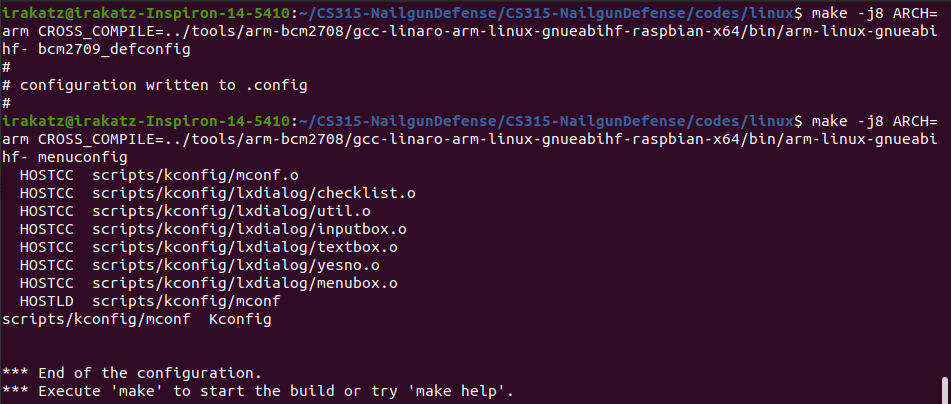
\includegraphics[width=0.8\linewidth]{sc1.png}
	\caption{Example of preparing configuration}
	\label{fig:sc1}
\end{figure}

Then, we will build the following things: (1) Image file (zImage) (2) 
device tree files (dtbs) (3) modules. In parameter 
\texttt{INSTALL\_MOD\_PATH}, you should provide the position of the 
compiled modules. (See in Figure~\ref{fig:sc2} and 
Figure~\ref{fig:sc3})


Be careful, the compilation may be stopped due to the lack of some 
essential tools (e.g., flex and bison), please download them with 
\texttt{apt-get}.

\begin{lstlisting}
mkdir ../modulespath

make -j8 ARCH=arm 
CROSS_COMPILE=tools/arm-bcm2708/gcc-linaro-arm-linux-gnueabihf-raspbian-x64\
/bin/arm-linux-gnueabihf- zImage dtbs modules

make -j8 ARCH=arm CROSS_COMPILE=tools/arm-bcm2708/gcc-linaro-arm-linux-gnueabihf-raspbian-x64\
/bin/arm-linux-gnueabihf- modules_install INSTALL_MOD_PATH=modulespath
\end{lstlisting}

\begin{figure}[H]
	\centering
	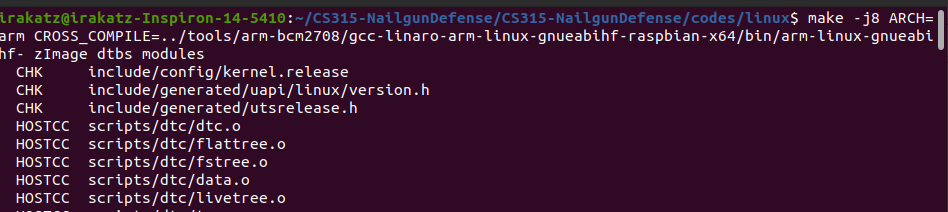
\includegraphics[width=0.8\linewidth]{sc2.png}
	\caption{Example of compiling kernel (1)}
	\label{fig:sc2}
\end{figure}

\begin{figure}[H]
	\centering
	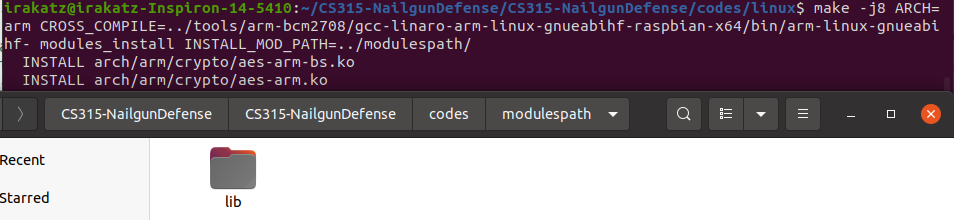
\includegraphics[width=0.8\linewidth]{sc3.png}
	\caption{Example of compiling kernel (2)}
	\label{fig:sc3}
\end{figure}

\subsubsection{Replace}

After you build the kernel, you can find the image in linux directory, which is 
\begin{lstlisting}
arch/arm/boot/zImage
\end{lstlisting}
\begin{figure}[H]
	\centering
	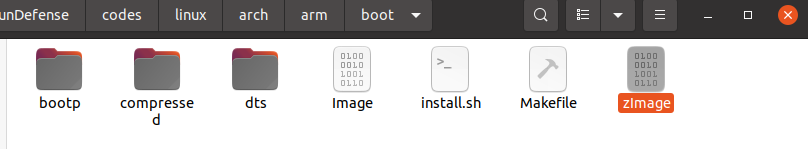
\includegraphics[width=0.8\linewidth]{sc4.png}
	\caption{Position of the zImage}
\end{figure}
And the device tree files in 
\begin{lstlisting}
arch/arm/boot/dts/
\end{lstlisting}

\begin{figure}[H]
	\centering
	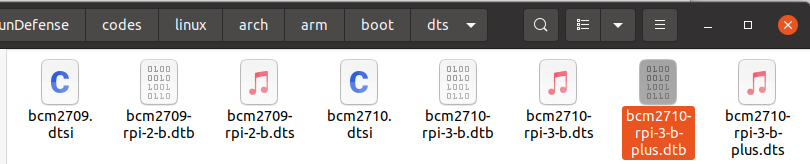
\includegraphics[width=0.8\linewidth]{sc5.png}
	\caption{Position of the device tree (for Raspberry Pi 3B+)}
\end{figure}
To replace the kernel and device tree files in the disk, we 
\begin{itemize}
	\item connect the Raspberry SD card (or USB) to your computer.
	\item make a linux kernel by script tool
	\item copy your kernel, device tree files and modules to the \texttt{boot} directory of the SD card
\end{itemize}


The following commands can be helpful. Note, you should provide the 
position of the boot directory (\texttt{BOOTDIR}) in your computer.

\begin{lstlisting}
./scripts/mkknlimg ./arch/arm/boot/zImage BOOTDIR/kernel7.img
cp BOOTDIR/kernel7.img BOOTDIR/kernel.img
cp ./arch/arm/boot/dts/bcm2710-rpi-3-b-plus.dtb BOOTDIR/
cp ./arch/arm/boot/dts/overlays/*.dtb* BOOTDIR/overlays/
\end{lstlisting}

\begin{figure}[H]
	\centering
	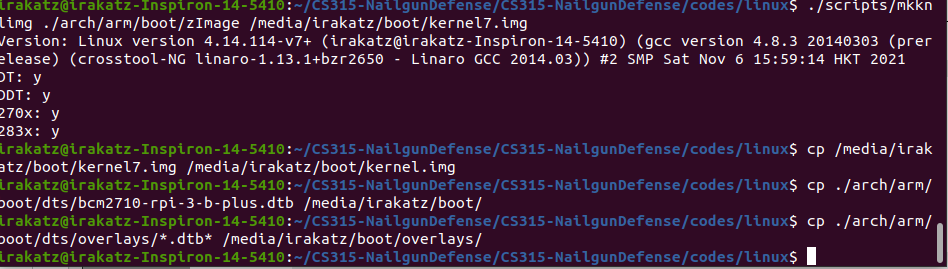
\includegraphics[width=0.8\linewidth]{sc6.png}
	\caption{Example of moving kenrel and dtb file}
\end{figure}


Once you replace the kernel and reboot it successfully, you can use the command "\texttt{uname -r}" to check the version of the kernel.

\begin{figure}[H]
	\centering
	\includegraphics[width=0.8\linewidth]{sc7.jpg}
	\caption{Example of successfully loading kernel}
\end{figure}



\subsubsection{About the Nailgun module}
You should build and install the Nailgun module with the compiled 
\texttt{modulespath}. or it would trigger a conflict.

Here we provide an example Nailgun attack(\texttt{Read\_SCR}). You 
download it 
and compile it on your Ubuntu, they copy the .ko file to Raspberry Pi.
Note, you should change the path of \texttt{CROSS\_COMPILE}, and 
\texttt{KERNELDIR} according to your \texttt{modulespath}.


\begin{lstlisting}
obj-m += nailgun.o


KERNELDIR := modulespath/lib/modules/4.14.114-v7+/build



all:
make ARCH=arm -C $(KERNELDIR) M=$(PWD) CROSS_COMPILE=tools/arm-bcm2708/gcc-linaro-arm-linux-gnueabihf-raspbian-x64\
/bin/arm-linux-gnueabihf- modules

clean:
make -C $(KERNELDIR) M=$(PWD) clean
\end{lstlisting}

\textbf{Question 1:(\textbf{20\%})} Can you prove that (1) you have 
replaced the 
kernel (with "uname -r" or other approaches), and (2) you have built 
the nailgun module with new headers? Please provide a figure. 


\textbf{Question 2:(\textbf{20\%})} Can you run the Nailgun Attack on 
your new 
kernel? Please provide a figure. You can use "dmesg" to show the 
execution result of Nailgun Attack. 

\subsection{Implementation of the Defense}

After you understand the steps of building a kernel, we start to 
implement the defense. As Mentioned in Section~\ref{sec:intro}, we 
leverage the Stage-2 translation to prevent the access of the 
memory-mapped interface for the debug registers. In Raspberry PI 3 
Module B+, \textbf{one address space} of the debug registers is 
\texttt{0x40030000 - 0x40030fff}.
Therefore, we restrict the access of this region from the kernel and 
user applications.


Note, we also provide the whole modified files in \texttt{modified} 
directory.


\subsubsection{Memory Reserve}

We reserve a 2MB memory region for the usage of Stage-2 translation. 
For instance, we select \texttt{0x32000000 - 0x321fffff}. Note that 
the region is large enough to store the page tables.

To reserve the memory, we should modify the corresponding device tree 
files. We insert the codes in the device tree files 
(arch/arm/boot/dts/bcm2710-rpi-3-b-plus.dts)
\begin{lstlisting}
	...
	aliases {
		serial0 = &uart1;
		serial1 = &uart0;
	};

//----------insert codes start------------
	reserved-memory {
		#address-cells = <1>;
		#size-cells = <1>;
		ranges;
		
		test_reserved: test@32000000{
			compatible = "test,test-memory";
			reg = <0x32000000 0x200000>;
			no-map;
		};
	};
//-----------insert codes end--------------
};

&gpio {
	...
\end{lstlisting}



Here we name the memory as \texttt{test@32000000}, while the start and size are provided in \texttt{reg}. The attribute \texttt{no-map} tells the kernel not to use the region when booting, so it protects the robustness of the system. However, if we do not implement any protection on this region, the kernel-level attacker can still access this region via some approaches.

\subsection{Codes of Defense}

\subsubsection{Architecture of the codes}

We begin to modify the source files of the Linux kernel. The source file of booting CPUs is \texttt{arch/arm/kernel/head.S}. You can find the \texttt{ENTRY(stext)}, which contains the configurations and codes for booting the primary CPU, and \texttt{ENTRY(secondary\_startup)} for booting the other CPUs. 

These codes have not implemented the Stage-2 translation, so we should achieve two goals: 
\begin{itemize}
	\item Creating a translation table, which entries are stored in the reserved memory (\texttt{0x32000000 - 0x321fffff})
	\item Configure the system registers to enable the Stage-2 translation
\end{itemize}

Since we are programming with the assembly language, we should use some regular registers to execute the add/load/store instructions. However, the kernel codes may occupy several registers to store some information (e.g., the branch address in the following steps). If we want to use them, we dump the values in the registers into memory and put them back later. It can be achieved by a temporarily used register.



Our code is placed between the comments \texttt{Our codes start} and \texttt{Our codes end}. We place the codes in two postions (primary and secondary CPUs), and you can also place your codes in other positions.
Note that the codes for primary CPU is not necessary in the Nailgun example, since it use core 1 (a secondary core) to map the debugging registers. In our example, we can only implement the Stage-2 translation on the secondary cores.

\begin{lstlisting}

ENTRY(stext)
ARM_BE8(setend	be )			@ ensure we are in BE8 mode

THUMB(	badr	r9, 1f		)	@ Kernel is always entered in ARM.
THUMB(	bx	r9		)	@ If this is a Thumb-2 kernel,
THUMB(	.thumb			)	@ switch to Thumb now.
THUMB(1:			)


#ifdef CONFIG_ARM_VIRT_EXT
bl	__hyp_stub_install
#endif

/*Our codes start*/
...
/*Our codes end*/

	@ ensure svc mode and all interrupts masked
safe_svcmode_maskall r9

...

ENTRY(secondary_startup)
/*
* Common entry point for secondary CPUs.
*
* Ensure that we're in SVC mode, and IRQs are disabled.  Lookup
* the processor type - there is no need to check the machine type
* as it has already been validated by the primary processor.
*/

ARM_BE8(setend	be)				@ ensure we are in BE8 mode

#ifdef CONFIG_ARM_VIRT_EXT
bl	__hyp_stub_install_secondary
#endif

/*Our codes start*/
...
/*Our codes end*/

	@ ensure svc mode and all interrupts masked
	safe_svcmode_maskall r9

mrc	p15, 0, r9, c0, c0		@ get processor id
bl	__lookup_processor_type
movs	r10, r5	
....

\end{lstlisting}


Here is an example, you can also use other general registers which is temporarily used.
You can find that we store the values of general registers in our reserved memory, since they are used in the next codes. To distinguish whether the register will be used or not, please read the source code of the kernel.

\begin{lstlisting}

//----------insert codes start------------
	/*Here we can use the regular registers r0
	*and we store the value r1, r2, r3, r4, r5
	*in our reserved memory
	*/
	ldr r0,=0x32000100
	str r2,[r0]
	ldr r0,=0x32000104
	str r3,[r0]
	ldr r0,=0x32000108
	str r4,[r0]
	ldr r0,=0x3200010C
	str r5,[r0]
	ldr r0,=0x32000110
	str r1,[r0]
	/*creating page table*/
	...
	/*configuring system registers*/
	...

	/*We finally fetch the values*/
	ldr r0,=0x32000100
	ldr r2,[r0]
	ldr r0,=0x32000104
	ldr r3,[r0]
	ldr r0,=0x32000108
	ldr r4,[r0]
	ldr r0,=0x3200010C
	ldr r5,[r0]
	ldr r0,=0x32000110
	ldr r1,[r0]
	mov r0,#0 //restore r0
//-----------insert codes end--------------

\end{lstlisting}

Now we can use the registers r0,r2,r3,r4,r5 to achieve the defense mechanism.

\subsubsection{Creating Translation Table}

\begin{figure}[htb]
	\centering
	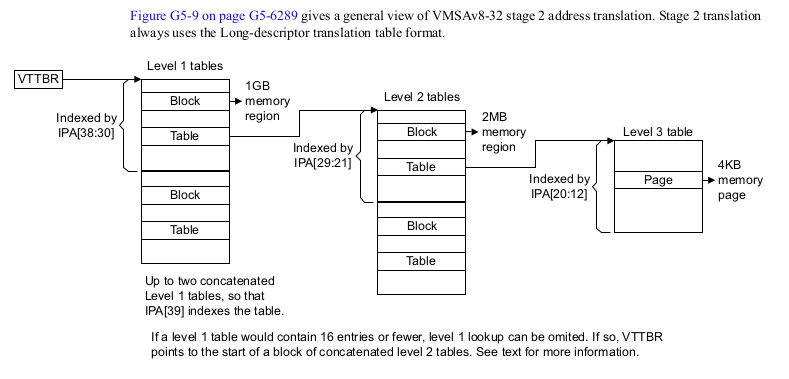
\includegraphics[width=1\linewidth]{vmsa.png}
	\caption{Stage-2 translation overview}
	\label{fig:vmsa}
\end{figure}

\vspace{10pt}
\textbf{Design of the Stage-2 translation table without defense}
\vspace{10pt}

In this step, we fill the translation table into the reserved region. 
Simply, we create a flat mapping between the IPA and PA of the whole address space (i.e., IPA == PA), and invalidate the mapping of both the debug registers (0x40030000 - 0x40030fff) and the Stage-2 translation table (0x32000000 - 0x321fffff).

A completed process of Stage-2 translation is separated into several levels (See in Figure~\ref{fig:vmsa}). For each level, the MMU will combine the input address with the entry (or the base address) at the current level, and get the address of the entry at the next level. 

\vspace{10pt}
\textbf{Structure of the table entry (descriptor)}
\vspace{10pt}

In Figure~\ref{fig:l1l2} and Figure ~\ref{fig:l3} (you can find the attributes in page G5-6290 and G5-6291),
each entry (or called as a descriptor) indicates the attributes (e.g., read permission, write permission, and access permission) of specific address space.
You can also find the partial component of the address related to the next-level entry (descriptor) or the output.
In particular, we care about the last two bits (bit[1:0]) of the entry, because they will tell us whether the translation should continue or stop. 

\begin{itemize}
	\item If we find a block or page, the translation is finished and will return the value.
	\item If we find an invalid entry, the translation is finished and will return a fault.
	\item If we find a table, the translation should continue.
\end{itemize}

\begin{figure}[htb]
	\centering
	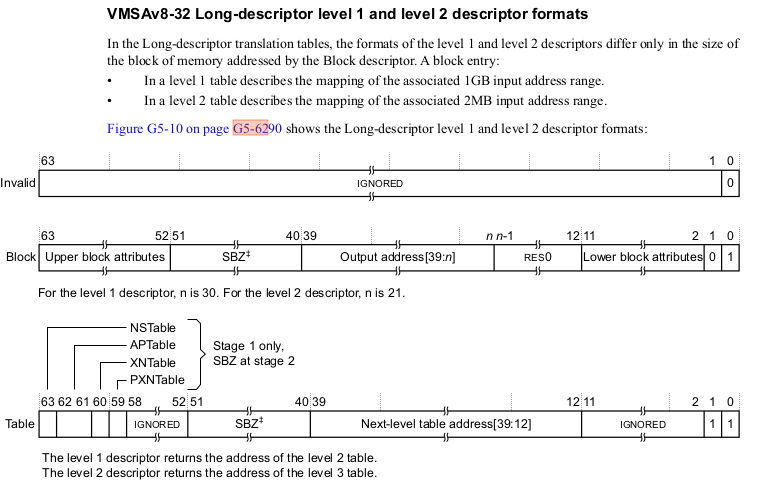
\includegraphics[width=1\linewidth]{l1l2.png}
	\caption{Structure of the level 1 \& 2 table entry (descriptor)}
	\label{fig:l1l2}
\end{figure}

\begin{figure}[htb]
	\centering
	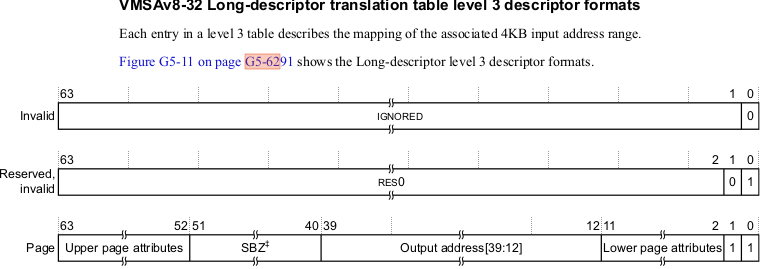
\includegraphics[width=1\linewidth]{l3.png}
	\caption{Structure of the level 3 table entry (descriptor)}
	\label{fig:l3}
\end{figure}

\vspace{10pt}
\textbf{Example of a table walk}
\vspace{10pt}


\begin{figure}[htbp]
	\centering
	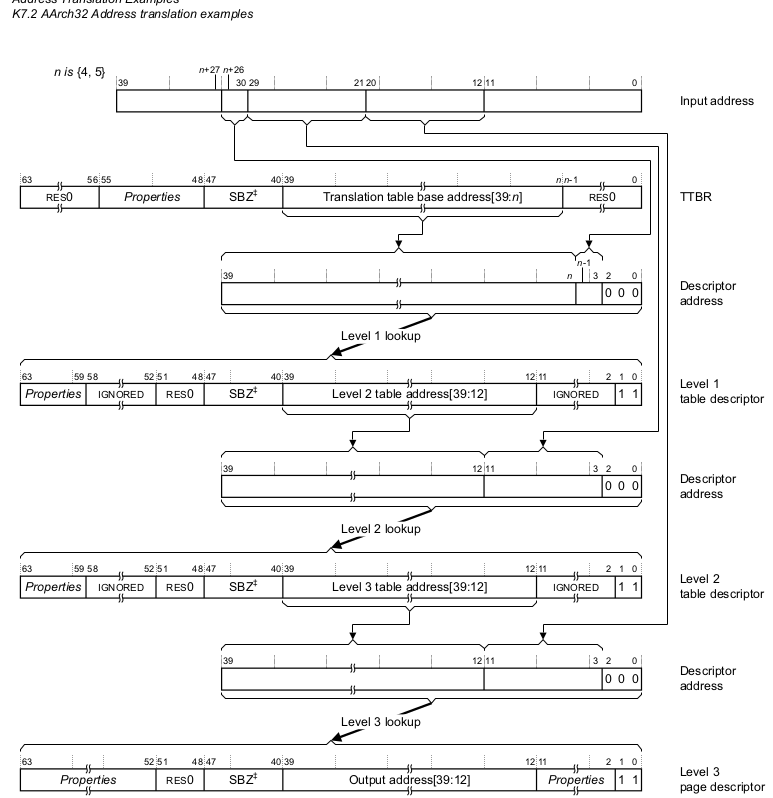
\includegraphics[width=1\linewidth]{k7.png}
	\caption{A translation example}
	\label{fig:k7}
\end{figure}

Here we provide an explanation of a translation starting at level 1 in Figure~\ref{fig:k7}. The corresponding Picture is provided in K7-8498 on the Armv8-A manual since Stage-2 translation implements the Long-descriptor format on the Aarch32 translation regime. Note that n=5 in the picture.

When MMU receives the translation requirement and the input IPA, it separates the IPA into 4 parts for the use of 3 levels.
In level 1, MMU combines the first part of input IPA and the base address of the Stage-2 translation table, then calculates the address of the level-1 entry.
The last two bits of the entry tell MMU whether the translation should continue, stop or return a fault.
If we continue the translation, MMU combines the second part of the IPA with the level-1 entry to get the region of the address of the level-2 entry. Finally, the level-3 entry tells the translation is valid or not. If the translation is valid, MMU combines the level-3 entry and the last component of the IPA (we can regard it as offset) to get the output result. 

\vspace{10pt}
\textbf{Example of the codes}
\vspace{10pt}

Here we assume the base address of the Stage-2 translation table as 0x32000000 and give an example of the Stage-2 translation for the region 0x80000000 - 0xbfffffff.

\begin{lstlisting}
ldr r0,=0x32000010
ldr r1,=0x800007FD
str r1,[r0]
add r0,	r0,	#4
ldr r1,=0x00400000
str r1,[r0]
\end{lstlisting}

The above codes mean that we store the entry 0x0040\_0000\_8000\_04FD in the region 0x32000010 - 0x32000017.
The last 2 bits indicate it as a block, which means the translation is finished here.
For a input IPA 0x81234567, the level 0 will combine 
bit[31:30] of IPA and bit[31:5] of the base address, then tell we to read the address 0x32000000 + (0x2 \textless \textless 3) = 0x32000010. Then, we get the level-1 entry by reading the value in this address.
With the bit[1:0] of this entry, we know it is a block (you can see Armv8-A manual on page G5-6290), not a table. So, our translation is finished, the output address is composed of two parts. Its bit[31:30] is from the entry, and bits[29:0] is from the input address. You can calculate it, and know that the value of the output address is the same as the input address.

\vspace{10pt}
\textbf{Not done yet}
\vspace{10pt}

Although the given example is easy to follow, we must configure the corresponding entries with smaller granules (i.e., the translation should not stop in level 1), since we consider protecting a 4KB region and a 2MB region, rather than a 1GB region.
To protect the 2MB region (it is the Stage-2 translation table, 0x32000000 - 0x321fffff), we should separate the 1GB region, 0x0 - 0x3fffffff into 512 2MB-sized regions. If we want to protect the 4KB region (it is the debug registers, 0x40030000 - 0x40030fff), we should separate the 2MB region, 0x40000000 - 0x401fffff into 512 4KB-sized regions. If not, we may protect an unexpected address space.


\vspace{10pt}
\textbf{Defense implementation}
\vspace{10pt}



Finally, we implement the protection of these regions by setting the last bit of the corresponding entry as 0, because in Figure~\ref{fig:l1l2} and ~\ref{fig:l3}, if the last bit (bit[0]) of an entry is 0, then it indicates an invalid entry. Therefore, when the MMU performs the Stage-2 translation for the access of these regions, it finally finds an invalid entry and returns a translation fault.

\subsubsection{Configuring the System Registers}
We consider to configure three significant registers: \texttt{VTTBR}, which indicates the base address of the Stage-2 translation; \texttt{HCR}, which enables the Stage-2 translation; \texttt{VTCR}, which indicates some attributes of the translation. If you are interested in the functions of such system registers, please read the reference manual.

First, we fill the \texttt{VTTBR} register, we directly put the start address (0x32000000) into the \texttt{BADDR} bits:

\begin{lstlisting}
ldr r0,=0x32000000
ldr r1,=0x0
mcrr p15, 6, r0, r1, c2
\end{lstlisting}


We then fill the \texttt{VTCR} register. We mainly care about the \texttt{T0SZ} and \texttt{SL0} bits, which indicate the region size and starting level, respectively:

\begin{lstlisting}
ldr r1,=0x80000040
mcr p15, 4, r1, c2, c1, 2
\end{lstlisting}

Finally, we configure the last bit (\texttt{VM}) of the \texttt{HCR} as 1 to enable the Stage-2 translation:

\begin{lstlisting}
mrc p15, 4, r0, C1, C1, 0 
orr	r0, r0, #0x1
mcr p15, 4, r0, C1, C1, 0
\end{lstlisting}

\textbf{Question 3:(30\%)} With the provided source codes, can you 
explain 
the process of traslating an IPA, \texttt{0x40030000}+"last 3 numbers 
of your student ID", to the same value of PA? (e.g., if your ID is 
12150073, then you should translate \texttt{0x40030073}).
In this question, you should mention the (1) address of each 
descriptor, and (2) value of each descriptor. 

\textbf{Question 4:(30\%)} With the provided source codes, can you 
explain 
the process of traslating an IPA, \texttt{0x40030000}+"last 7 numbers 
of your student ID", to the same value of PA? (e.g., if your ID is 
12150073, then you should translate \texttt{0x42150073}).
In this question, you should mention the (1) address of each 
descriptor, and (2) value of each descriptor.





